% !TEX TS-program = pdflatex
\documentclass[letterpaper, 10pt, conference]{IEEEtran} %Document's type specification
\IEEEoverridecommandlockouts % This command is only needed if you want to use the \thanks command
\usepackage[english]{babel} %Package of english language handling
\usepackage[utf8]{inputenc} %Package to include characters with accents
\usepackage{amsmath, amssymb, amsfonts} %Package of math equations, symbols, etc.
\usepackage{graphicx} %Package of figures handling
\usepackage{xcolor} %Package of colors handling
\usepackage{hyperref} %Package for hyperlinks handling such internet links and document's direct links such in table of contents

\def \IEEEkeywordsname{Keywords}
\def \IEEEproofname{Proof}

\def \BibTeX{
	{\rm B\kern-0.05em{\sc i\kern-0.025em b}\kern-0.08em
	T\kern-0.1667em\lower0.7ex\hbox{E}\kern-0.125emX}
}

\title{Paper Title \\
	{\footnotesize \textsuperscript{*}Note: The subtitles aren't captured in Xplore and they shouldn't be used}
	\thanks{It may identify the applicable funding agency here. If there isn't anyone, you may delete this.}
}

\author{
	\IEEEauthorblockN{1\textsuperscript{st} Name and Surname}
	\IEEEauthorblockA{\textit{Dept. Name of Organization (of Aff.)} \\
		\textit{Name of Organization (of Aff.)} \\
		City, Country \\
		\href{John.A.Doe@ieee.org}{Email Address}
	}
	\and
	\IEEEauthorblockN{2\textsuperscript{nd} Name and Surname}
	\IEEEauthorblockA{\textit{Dept. Name of Organization (of Aff.)} \\
		\textit{Name of Organization (of Aff.)} \\
		City, Country \\
		\href{John.A.Doe@ieee.org}{Email Address}
	}
	\and
	\IEEEauthorblockN{3\textsuperscript{rd} Name and Surname}
	\IEEEauthorblockA{\textit{Dept. Name of Organization (of Aff.)} \\
		\textit{Name of Organization (of Aff.)} \\
		City, Country \\
		\href{John.A.Doe@ieee.org}{Email Address}
	}
	\and
	\IEEEauthorblockN{4\textsuperscript{th} Name and Surname}
	\IEEEauthorblockA{\textit{Dept. Name of Organization (of Aff.)} \\
		\textit{Name of Organization (of Aff.)} \\
		City, Country \\
		\href{John.A.Doe@ieee.org}{Email Address}
	}
	\and
	\IEEEauthorblockN{5\textsuperscript{th} Name and Surname}
	\IEEEauthorblockA{\textit{Dept. Name of Organization (of Aff.)} \\
		\textit{Name of Organization (of Aff.)} \\
		City, Country \\
		\href{John.A.Doe@ieee.org}{Email Address}
	}
	\and
	\IEEEauthorblockN{6\textsuperscript{th} Name and Surname}
	\IEEEauthorblockA{\textit{Dept. Name of Organization (of Aff.)} \\
		\textit{Name of Organization (of Aff.)} \\
		City, Country \\
		\href{John.A.Doe@ieee.org}{Email Address}
	}
}

\begin{document}
	\maketitle
	
	\begin{abstract}
		This document is a sample of the format defined by IEEE Standards to write representative articles of a performed project. Authors must follow the instructions, including format and paper size to keep the publishing's standard. This document may be interpreted as a set of instructions to write the article or as a template to make it. As you may have noticed, this first section is given to generate a very short and high scale summary of the project's scope and results. *CRITICAL: Do not use symbols, special characters, footnotes, or math equations at document's title or abstract.
	\end{abstract}
	
	\begin{IEEEkeywords}
		IEEE, component, formatting, style, insert, references
	\end{IEEEkeywords}
	
	\section{Introduction} \label{sectionIntroduccion}
	This document is a model and it has instructions for {\LaTeX}. It's important to observe the page limits of the conference document type.
	
	The IEEE \emph{(Institute of Electrical and Electronics Engineers)} is a non-profit organization whose objective is to promote the creativity, development, integration, applicability and the sharing of advances in information technologies and sciences in general for the humanity and the same professionals' benefit \cite{bibliographicReference1}, besides, it's one of the most important organizations in the creation of standards worldwide, and in particular, it has defined some standards of universal kind for the scientific articles' construction, projects and research results reports, widely used in engineering and science, as part of the academic training stage in universities, research activities, etc.
	
	The purpose with which this template is reviewed and improved is to make it easier for users to get this resource and its usability when they build their article, so that they don't have to worry about adjusting margins, section enumerations, the texts' format and other aspects directly related to the style of the document or the texts' format.
	
	The IEEEtran.cls' class file, which is outside the main Document.tex' file, is the basis on which the format and the IEEE's fundamental standards are applied in the Document.pdf's file generated on the main Document.tex' file, that class file has been implemented and updated by Gerry Murray, Silvano Balemi, Jon Dixon, Peter Nuchter, Juergen von Hagen, and Michael Shell, this last one is the current responsible for this class file's maintaining for future modifications and updates \cite{bibliographicReference2}.
	
	Despite the constant IEEE standards' updates in almost any industry, there is an issue about the maximum size that may be occupied in the document for the graphic elements such as images, statistical charts, tables, maps, etc., because the IEEE standards' document style considers the use of two columns of text and this may hinder the readability of those graphic elements for the readers, from this observation, this same template is alternatively available but with text in only one column. so that the other rules of the document style are kept and to allow to these graphic elements to occupy the most of the page's width and to improve their readability for the readers.
	
	\section{Ease of Use} \label{sectionEaseOfUse}
	\subsection{Free Access to the Template} \label{subsectionFreeAccessToTheTemplate}
	To reuse this template, this english version for two columns may be found for its later edition available in Overleaf at \href{https://es.overleaf.com/read/yvwjymdknjjm}{https://es.overleaf.com/read/yvwjymdknjjm} or locally with the TexStudio's IDE in the Github repository at \href{https://github.com/mamurciac/DocumentsTemplates_PublicVersion/tree/main/IEEE%20Report%20%5BEnglish%20with%20Double%20Column%5D}{https://github.com/mamurciac/DocumentsTemplates\_ PublicVersion/tree/main/IEEE\%20Report\%20\%5BEnglish\% 20with\%20Double\%20Column\%5D} for its later download and edition.
	
	Also, the following versions are available (according to the language and number of columns):
	\begin{itemize}
		\item English to a single column, it's available in Overleaf at \href{https://es.overleaf.com/read/gvyvqvsdkzfy}{https://es.overleaf.com/read/gvyvqvsdkzfy} or locally in the Github repository at \href{https://github.com/mamurciac/DocumentsTemplates_PublicVersion/tree/main/IEEE%20Report%20%5BEnglish%20with%20Single%20Column%5D}{https://github.com/mamurciac/DocumentsTemplates\_ PublicVersion/tree/main/IEEE\%20Report\%20\%5BEnglish \%20with\%20Single\%20Column\%5D}.
		\item Spanish to double column, it's available in Overleaf at \href{https://es.overleaf.com/read/dntrzbbwdxkv}{https://es.overleaf.com/read/dntrzbbwdxkv} or locally in the Github repository at \href{https://github.com/mamurciac/DocumentsTemplates_PublicVersion/tree/main/IEEE%20Report%20%5BSpanish%20with%20Double%20Column%5D}{https://github.com/mamurciac/DocumentsTemplates\_ PublicVersion/tree/main/IEEE\%20Report\%20\%5BSpanish \%20with\%20Double\%20Column\%5D}.
		\item Spanish to a single column, it's available in Overleaf at \href{https://es.overleaf.com/read/rtrmjjvkhszt}{https://es.overleaf.com/read/rtrmjjvkhszt} or locally in the Github repository at \href{https://github.com/mamurciac/DocumentsTemplates_PublicVersion/tree/main/IEEE%20Report%20%5BSpanish%20with%20Single%20Column%5D}{https://github.com/mamurciac/DocumentsTemplates\_ PublicVersion/tree/main/IEEE\%20Report\%20\%5BSpanish \%20with\%20Single\%20Column\%5D}.
	\end{itemize}
	
	\subsection{Maintaining the Integrity of the Specifications} \label{subsectionMaintainingTheIntegrityOfTheSpecifications}
	The IEEEtran.cls class file is used to format your paper and style the text. All margins, column widths, line spaces, and text fonts are prescribed; please don't alter them. You may note peculiarities, for example, the head margin measures proportionately more than is customary. This measurement and others are deliberate, using specifications that anticipate your work as one part of the entire process, and not as an independent document. Please don't revise any of the current designations.
	
	\section{Prepare Your Paper Before Styling} \label{sectionPrepareYourPaperBeforeStyling}
	Before you begin to format your work, first, it's recommended to write and to save the content as a separate text file, to complete all content and organizational editon before formatting. Also, it's recommended to consider the sections \ref{subsectionAbbreviationsAndAcronyms}--\ref{subsectionSomeCommonMistakes} below for more information about review, orthography and grammar.
	
	Please keep your text and graphic files separate until the text has been formatted and properly styled, and don't number text heads because {\LaTeX} will do it automatically.
	
	\subsection{Abbreviations and Acronyms} \label{subsectionAbbreviationsAndAcronyms}
	It's recommended to define abbreviations and acronyms the first time they are used in the text, even after they have been defined at the abstract. It doesn't have to define abbreviations such as IEEE, SI, MKS, CGS, ac, dc, or rms, and please don't use abbreviations at the title or heads unless they are unavoidable.
	
	\subsection{Units} \label{subsectionUnits}
	\begin{itemize}
		\item It's recommended to use the IS' \emph{(International System)} units, which in particular it contains the MKS \emph{(Meter, kilogram and second)}, or CGS' \emph{(Cegesimal System)} units as primary measure units, the SI units are especially recommended.
		\item The english units can be used as secondary measure units (in parentheses) though an exception would be the use of english units as identifiers in commerce, such as ``3.5-inch disk drive''.
		\item It isn't recommended to mix SI and CGS units, such as current in amps and magnetic field in oersteds, this often leads to confusion because the equations don't balance them dimensionally. If mixed units must be used, the units must be clearly indicated for each one quantity used in a math equation.
		\item The full spelling with unit abbreviations mustn't be mixed, for example, you can use ``Wb/m\textsuperscript{2}'' or ``webers per square meter'', but not ``webers/m\textsuperscript {2}'', nevertheless, the units may be spelled when they appear in the text, for example, it is recommended to mention: ``. . . some henrys'', but not ``. . . some H''.
		\item It's recommended to use a zero before decimal points, for example ``0.25'' but not ``.25'', and it's also recommended to use ``cm\textsuperscript{3}'', instead of ``cc'' for volume units.
	\end{itemize}
	
	\subsection{Equations} \label{subsectionEquations}
	It's recommended to number numerical equations consecutively. To make the math equations more compact, you can use slashes (~/~), the exponential function, or appropriate exponents.
	
	It's recommended to italicize the symbols in roman alphabet for quantities and variables, but not the symbols in greek alphabet, it's also recommended to use an em dash instead of a hyphen for a minus sign.
	
	The following item is an example of an equation:
	\begin{equation}
		a + b = \gamma
		\label{exampleOfEquation}
	\end{equation}
	
	For recognition of some variables and possibly some unknown constants, it's recommended to ensure that the symbols in each equation have been defined before or immediately after the equation.
	
	When the equations are mentioned in the text, that is, when they are part of a sentence, it's recommended to use ``\eqref{exampleOfEquation}'', but not ``Ec.~\eqref{exampleOfEquation}'' neither ``equation \eqref{exampleOfEquation}'', except at the beginning of a sentence, for example, ``Equation \eqref{exampleOfEquation} is . . .''.
	
	\subsection{{\LaTeX} Specific Advices} \label{subsectionLatexSpecificAdvices}
	Please use ``soft'' cross references (e.g., \verb|\eqref{exampleOfEquation}|) instead of ``hard'' cross-references (e.g., \verb|(1)|), this will allow you to combine sections, to add equations or to change the order of figures or quotes without having to go through the file line by line and without mixing references of some elements with others; for example, to avoid mixing figure references with table references or even section references that are part of the document's structure.
	
	It's recommended not to use the equation environment \verb|{eqnarray}|, but to use the environments \verb|{align}| or \verb|{IEEEeqnarray}| instead, this is requested because the environment \verb|{eqnarray}| leaves unsightly spaces around relationship symbols and around some other symbols.
	
	Please note that the environment \verb|{subequations}| in {\LaTeX} will increment the main equations' counter, even when no equation numbers are displayed; if this is forgotten, an article may be written in which the equation numbers jump from (17) to (20) for example, indicating possible missing equations or failures in the enumeration of these elements.
	
	{\BibTeX} doesn't work by magic, it doesn't get the bibliographic data from thin air but from .bib files. If {\BibTeX} is used to produce a bibliography, it must be sent via .bib files.
	
	{\LaTeX} may not read your mind, if you assign the same label to a subsection and a table, you might find that for example Table I has been cross referenced as Table IV-BibliographicReference3.
	
	{\LaTeX} doesn't have precognitive abilities, if you put a \verb|\label| command before the command that updates the counter it's supposed to be using it, the label will pick up the latest counter to be cross referenced instead; in particular, a \verb|\label| command shouldn't go located before the title of a figure or table.
	
	Please don't use the \verb|\nonumber| command inside the \verb|{array}| environment, this won't stop the equation numbers inside the \verb|{array}| command (There won't be any anyway) and it might stop at an unwanted equation number in the surrounding equation.
	
	\subsection{Some Common Mistakes}\label{subsectionSomeCommonMistakes}
	\begin{itemize}
		\item The word ``data'' is in plural, not in singular.
		\item The subscript for the vacuum's permeability $\mu_{0}$, and other common scientific constants, is zero with subscript formatting, not a lowercase letter ``o''.
		\item In american english, the commas, semicolons, periods, question and exclamation marks are located within quotation marks only when a complete thought or name is cited, such as a title or a full quotation. When the quotation marks are used, instead of a bold or italic typeface to highlight a word or phrase, the punctuation must appear outside of the quotation marks. A phrase or statement between parentheses at the end of a sentence is punctuated outside of the closing parenthesis (like this). (A sentence between parentheses is punctuated within the parentheses.)
		\item A graph within a graph is an ``inset'', not an ``insert''.
		\item Don't use the word ``essentially'' to mean ``approximately'' or ``effectively''.
		\item In your work's title, if the words ``that uses'' may replace accurately the word ``using'', then capitalize the letter ``u''; else, the word keeps it lowercased.
		\item It's recommended to be aware of the different meanings of the quasihomophone words ``affect'' and ``effect'', ``complement'' and ``compliment'', ``discreet'' and ``discrete'', ``principal'' and ``principle''.
		\item Don't confuse ``imply'' and ``infer''.
		\item There isn't a period after the word ``et'' in the Latin abbreviation ``et al.'', this Latin expression non-abbreviated is \emph{``et alii''} that means ``and others'' in English language.
		\item The Latin expression ``i.e.'' non-abbreviated is \emph{``id est''} that means ``is to say'' in English language.
		\item The Latin expression ``e.g.'' non-abbreviated is \emph{``exempli gratia''} that means ``for example'' in English language.
	\end{itemize}
	
	An excellent style manual for science writers is in \cite{bibliographicReference3}.
	
	\subsection{Authors and Affiliations} \label{subsectionAuthorsAndAffiliations}
	\textbf{The class file is designed for, but not limited to six authors.} A  minimum of one author is required for all conference articles. The author names should be listed starting from left to right and then moving down to the next line, this is the author sequence that will be used in future citations and by indexing services. The names shouldn't be listed in columns or grouped by affiliation, besides, it's recommended to keep affiliations as brief as possible (for example, don't differentiate among departments of the same organization).
	
	\subsection{Identify the Headings} \label{subsectionIdentifyTheHeadings}
	The headings or heads are organizational resources that guide the reader through the work. There are two heads types: component heads and text heads.
	
	The component headings identify the different components of the work and aren't topically subordinate to each other. The examples include Acknowledgments and References, and for these, the correct style to use is ``Heading 5''. It's recommended to use ``figure caption'' for the figure captions, and ``table head'' for the table titles. The initial headings, such as ``Abstract'', require a style (in this case, italic) to be applied  in addition to the style provided by the dropdown menu to differentiate the head from the text.
	
	The text headings organize the topics on a relational and hierarchical basis, for example, the work's title is the primary text head because all the subsequent material relates and elaborates it on this topic. If there are two or more subtopics, the next level head (with uppercase Roman numbers) should be used and, conversely, if there aren't at least two subtopics, then no subheads should be introduced.
	
	\subsection{Figures and Tables} \label{subsectionFiguresAndTables}
	\paragraph{Positioning Figures and Tables} It's recommended to place figures and tables at the top and bottom of the columns, in addition to avoiding to place them in the middle of the columns. The large figures can occupy both columns.
	
	The figure titles must be below the figures, the table headings must appear above the tables, it's recommended to insert figures and tables after they are cited in the text. You may use the abbreviation ``Fig.~\ref{exampleOfFigure}'', even at the beginning of a sentence.
	
	\begin{table}[htbp]
		\caption{Table Type Styles}
		\begin{center}
			\begin{tabular}{|c|c|c|c|}
				\hline
				\textbf{Table} & \multicolumn{3}{|c|}{\textbf{Table Column Head}} \\
				\cline{2-4}
				\textbf{Head} & \textbf{\textit{Table column subhead}} & \textbf{\textit{Subhead}} & \textbf{\textit{Subhead}} \\
				\hline
				copy & More table copy$^{\mathrm{a}}$ & & \\
				\hline
				\multicolumn{4}{l}{$^{\mathrm{a}}$Sample of a Table footnote.}
			\end{tabular}
			\label{exampleOfTable}
		\end{center}
	\end{table}
	
	\begin{figure}[htbp]
		\centerline{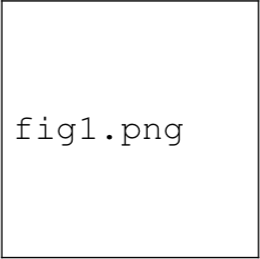
\includegraphics{Figures/Figure1.png}}
		\caption{Example of a figure caption.}
		\label{exampleOfFigure}
	\end{figure}
	
	\paragraph{Figure Labels} It's recommended to use the font Times New Roman with 8 points for figure labels. The words may be used instead of symbols or abbreviations when writing figure axis labels to avoid confusions to the reader; for example, to write the quantity ``Magnetization'', or ``Magnetization, M'', but not just ``M''. If the units are included on the label, they must be represented between parentheses. The axes shouldn't be labeled with units only; for example, you may write ``Magnetization (A/m)'' or ``Magnetization \{A[m(1)]\}'', but not just ``A/m'', besides, it's recommended not to label axes with a ratio of quantities and units, for example, you may write ``Temperature (K)'', but not ``Temperature/K''.
	
	\section*{Acknowledgments} \label{sectionAcknowlegments}
	It's recommended to avoid the rigid expression ``one of us (R. B. G.) thanks $\ldots$'', instead, you may use ``R. B. G. thanks $\ldots$''. The sponsor acknowledgments are requested to be placed in the unnumbered footnote at the bottom of the first page.
	
	\section*{Including Quotes and References in the Text} \label{sectionIncludingQuotesAndReferencesInTheText}
	Please number the citations consecutively between parentheses \cite{bibliographicReference4}, the sentence punctuation follows the parentheses \cite{bibliographicReference5}. Please indicate simply the reference number, as in \cite{bibliographicReference6}---instead of ``Ref. \cite{bibliographicReference6}'' neither ``reference \cite{bibliographicReference6}'' except at the beginning of a sentence, for example, ``Reference \cite{bibliographicReference6} was the first $\ldots$''
	
	Please number footnotes separately in superscripts, place the current footnote at the bottom of the column in which it was cited. It's recommended not to put footnotes at the abstract or in the references' list, neither use letters for table footnotes.
	
	Unless there are six authors or more, please give all authors' names without exception; please don't use ``et al.'' to skip missing authors of indicate. The papers that haven't been published, even if they have been submitted for publication, should be cited as ``unpublished'' \cite{bibliographicReference7}, the papers that have been accepted for publication should be cited as ``in press'' \cite{bibliographicReference8}.
	
	It must capitalize only the first word at the paper's title, except for proper nouns and elements' symbols.
	
	For papers published in translation journals, please give the English citation first, followed by the original foreign-language citation \cite{bibliographicReference9}.
	
	\section*{Bibliographic References Construction} \label{sectionBibliographicReferencesConstruction}
	In all research articles, project results reports, among others, the ethical, responsible and legitimate information's use gotten from any bibliographic resource must be made. When the bibliographical references are included, the ideas and information of works by other authors are identified, as well as the giving recognition to them for the information extracted from those resources that contribute directly to the construction of the article or report \cite{bibliographicReference10}.
	
	When the bibliographic references are indicated, this must be done in a structured way, is to say, there is an IEEE's standard defined, as well as in APA \emph{(American Psychological Association)}, ICONTEC \emph{(Colombian Institute of Technical Standards) } or ACM \emph{(Association for Computing Machinery)} to write the bibliographic references and thus to identify each bibliographic resource used from attributes such as authors' names, work's title, country of production, dates of publication, institutions or companies, etc.
	
	Next, the structure to write bibliographical references based on IEEE standards id indicated, depending on the type of resource or source:
	\begin{itemize}
		\item \textbf{\emph{Book:}} Initials and Surname(s) of the author(s), \textit{Title of the book in italics}. Edition. Place of publication: Editorial/Publisher, Year of publication.
		\item \textbf{\emph{Undergraduate, magister or doctoral thesis:}} Initials and Surname(s) of the author(s), ``Title of the thesis or project'', Kind of document (doctoral thesis , magister thesis, etc.), Department, Academic Institution (abbreviated), City, State abbreviated, Year.
		\item \textbf{\emph{Journal article:}} Initials and Surname(s) of the author(s), ``Title of article'', \textit{Abbreviated journal name in italics}, volume (abbreviated vol.), abbreviated number (no.) pages (abbreviated pp.), Month and Year.
		\item \textbf{\emph{Lecture notes:}} Initials and Surname(s) of the author(s) (if it's applicable), ``Title of the notes or subject'', Lecture notes for code of the subject, Department, Institution or University, season/semester and year.
		\item \textbf{\emph{From Web:}} Initials and Surname(s) of the author(s), Date of publication in format (year, month and day). Title (edition) [Type of media, usually Online]. Available: Url/Link.
	\end{itemize}
	
	Next, some samples about bibliographic references with IEEE standards are shown:
	\begin{itemize}
		\item \textbf{\emph{IEEE reference example of a book:}} R. G. Gallager. \textit{Principles of Digital Communication}. New York: Cambridge University Press, 2008.
		\item \textbf{\emph{IEEE reference example of a thesis:}} H. Zhang, ``Delay-insensitive networks'', Magister thesis, Waterloo University, Waterloo, ON, Canada, 1997.
		\item \textbf{\emph{IEEE reference example of a journal article:}} G. Liu, K. Y. Lee, and H. F. Jordan, ``TDM and TWDM de Brujin networks and suffflenets for optical communications'', \textit{IEEE Transactions on Computers}, vol. 46, pp. 695-701, June 1997.
		\item \textbf{\emph{IEEE reference example of lecture notes:}} ``Signal integrity and interconnects for high-speed applications'', lecture notes for ECE497-JS, Department of Electric and Computing Engineering, University of Illinois at Urbana-Champaign, Winter 1997.
		\item \textbf{\emph{IEEE reference example of a webpage:}} J. Jones. (1991, May 10). Networks (2nd ed.) [Online]. Available: \href{http://www.atm.com}{http://www.atm.com}.
	\end{itemize}
	
	\begin{thebibliography}{00}
		\bibitem{bibliographicReference1} (2021, December 29). Institute of Electrical and Electronics Engineers [Online]. Available: \href{https://es.wikipedia.org/wiki/Institute_of_Electrical_and_Electronics_Engineers}{https://es.wikipedia.org/wiki/Institute\_of\_Electrical\_and\_Electronics\_ Engineers}.
		\bibitem{bibliographicReference2} (2015, August 26). CTAN Comprehensive TEX Archive Network [Online]. Available: \href{https://www.ctan.org/tex-archive/macros/latex/contrib/IEEEtran/}{https://www.ctan.org/tex-archive/macros/latex/contrib/IEEEtran/}.
		\bibitem{bibliographicReference3} M. Young, The Technical Writer's Handbook. Mill Valley, CA: University Science, 1989.
		\bibitem{bibliographicReference4} G. Eason, B. Noble, and I. N. Sneddon, ``On certain integrals of Lipschitz-Hankel type involving products of Bessel functions,'' Phil. Trans. Roy. Soc. London, vol. A247, pp. 529--551, April 1955.
		\bibitem{bibliographicReference5} J. Clerk Maxwell, A Treatise on Electricity and Magnetism, 3rd ed., vol. 2. Oxford: Clarendon, 1892, pp. 68--73.
		\bibitem{bibliographicReference6} I. S. Jacobs and C. P. Bean, ``Fine particles, thin films and exchange anisotropy,'' in Magnetism, vol. III, G. T. Rado and H. Suhl, Eds. New York: Academic, 1963, pp. 271--350.
		\bibitem{bibliographicReference7} K. Elissa, ``Title of paper if known,'' unpublished.
		\bibitem{bibliographicReference8} R. Nicole, ``Title of paper with only first word capitalized,'' J. Name Stand. Abbrev., in press.
		\bibitem{bibliographicReference9} Y. Yorozu, M. Hirano, K. Oka, and Y. Tagawa, ``Electron spectroscopy studies on magneto-optical media and plastic substrate interface,'' IEEE Transl. J. Magn. Japan, vol. 2, pp. 740--741, August 1987 [Digests 9th Annual Conf. Magnetics Japan, pp. 301, 1982].
		\bibitem{bibliographicReference10} (2022, March 10). Citas y elaboración de bibliografía: el plagio y el uso ético de la información: Estilo IEEE [Online]. Available: \href{https://biblioguias.uam.es/citar/estilo_ieee}{https://biblioguias.uam.es/citar/estilo\_ieee}.
	\end{thebibliography}
	
	\vspace{12pt}
	\color{red}
	The IEEE's conference templates contain guidance text to compose and to format conference papers. Please ensure that all template text is removed from your conference paper prior to submission to the conference. If it fails to remove the template text from your paper, it may result that your paper isn't published.
\end{document}